% !TeX program = xelatex
\documentclass[11pt,a4paper]{article}

% -------------------------------------------------
% Packages
% -------------------------------------------------
\usepackage{kotex}
\usepackage{fontspec}
\usepackage{amsmath,amssymb,bm,mathtools}
\usepackage[left=24mm,right=24mm,top=23mm,bottom=25mm]{geometry}
\usepackage{booktabs,array}
\usepackage{enumitem}
\usepackage{setspace}
\usepackage{xcolor}
\usepackage{tikz}
\usetikzlibrary{positioning,arrows.meta,calc,fit}
\usepackage[most]{tcolorbox}
\usepackage{listings}
\usepackage{hyperref}
\usepackage{fancyhdr}

\setstretch{1.14}
\setlength{\parindent}{0pt}
\setlength{\parskip}{0.55em}

% -------------------------------------------------
% Colors and boxes
% -------------------------------------------------
\definecolor{deepblue}{RGB}{34,71,120}
\definecolor{softblue}{RGB}{239,246,253}
\definecolor{softgray}{RGB}{246,247,249}
\definecolor{softgreen}{RGB}{239,249,242}
\definecolor{softyellow}{RGB}{255,249,229}
\definecolor{codegray}{RGB}{248,248,248}

\newtcolorbox{keybox}[1][]{
  colback=softblue,
  colframe=deepblue,
  boxrule=0.7pt,
  arc=2mm,
  title=#1,
  fonttitle=\bfseries
}

\newtcolorbox{thinkbox}[1][]{
  colback=softyellow,
  colframe=orange!70!black,
  boxrule=0.6pt,
  arc=2mm,
  title=#1,
  fonttitle=\bfseries
}

\newtcolorbox{remarkbox}[1][]{
  colback=softgray,
  colframe=black!45,
  boxrule=0.5pt,
  arc=2mm,
  title=#1,
  fonttitle=\bfseries
}

\newtcolorbox{mlbox}[1][]{
  colback=softgreen,
  colframe=green!45!black,
  boxrule=0.6pt,
  arc=2mm,
  title=#1,
  fonttitle=\bfseries
}

% -------------------------------------------------
% Code style
% -------------------------------------------------
\lstdefinestyle{pythonstyle}{
  language=Python,
  backgroundcolor=\color{codegray},
  basicstyle=\ttfamily\small,
  keywordstyle=\bfseries,
  commentstyle=\itshape\color{black!60},
  stringstyle=\color{black!75},
  numbers=left,
  numberstyle=\tiny\color{black!55},
  numbersep=8pt,
  frame=single,
  rulecolor=\color{black!25},
  breaklines=true,
  showstringspaces=false,
  tabsize=4,
  columns=fullflexible,
  keepspaces=true
}
\lstset{style=pythonstyle}

% -------------------------------------------------
% Math commands
% -------------------------------------------------
\newcommand{\R}{\mathbb{R}}
\newcommand{\grad}{\nabla}
\newcommand{\vect}[1]{\bm{#1}}
\newcommand{\T}{^{\mathsf T}}
\newcommand{\dd}{\,\mathrm d}
\newcommand{\loss}{\mathcal{L}}

% -------------------------------------------------
% Header / footer
% -------------------------------------------------
\pagestyle{fancy}
\fancyhf{}
\lhead{Introduction to Deep Learning and Practice}
\rhead{Chain Rule and Backpropagation}
\cfoot{\thepage}
\renewcommand{\headrulewidth}{0.4pt}
\setlength{\headheight}{14pt}

\hypersetup{
  colorlinks=true,
  linkcolor=deepblue,
  urlcolor=deepblue
}

% -------------------------------------------------
% Document
% -------------------------------------------------
\begin{document}

\begin{center}
{\LARGE\bfseries 합성함수 미분법에서 Backpropagation까지}\\[0.35em]
{\Large Chain Rule $\rightarrow$ Multivariable Chain Rule $\rightarrow$ Linear Regression}\\[0.8em]
{\large 딥러닝개론및연습 --- 주차 강의노트 초안}
\end{center}

\vspace{0.4em}

\begin{keybox}[이번 주의 핵심 질문]
딥러닝에서 학습한다는 것은 결국 손실함수 $L$을 모델 파라미터에 대해 미분하고,
그 미분값을 이용하여 파라미터를 수정하는 과정이다. 그렇다면 수많은 함수가 반복적으로
합성된 신경망에서
\[
\frac{\partial L}{\partial \theta}
\]
를 어떻게 체계적으로 계산할 수 있을까?

이번 주에는 그 출발점이 되는 \textbf{chain rule}을 일변수에서 다변수로 확장하고,
가장 단순한 학습모델인 선형회귀를 계산 그래프로 다시 해석하여
\textbf{forward propagation과 backward propagation의 원형}을 직접 유도하고 구현한다.
\end{keybox}

\subsection*{학습목표}
이 주차가 끝나면 다음을 설명하고 직접 계산할 수 있어야 한다.
\begin{enumerate}[label=\arabic*.]
\item 합성함수와 chain rule을 ``변화율의 전달''이라는 관점에서 설명한다.
\item 편미분, gradient, Jacobian의 의미를 구분한다.
\item 다변수 chain rule을 scalar form과 matrix form으로 표현한다.
\item 계산 그래프(computational graph)에서 forward와 backward의 의미를 설명한다.
\item 선형회귀의 MSE loss에 대해 $\partial L/\partial w$, $\partial L/\partial b$를 chain rule로 유도한다.
\item 위 유도식을 NumPy로 직접 hard coding하여 gradient descent를 수행한다.
\end{enumerate}

\begin{remarkbox}[권장 시간 구성]
\textbf{1차시(약 50분):} 일변수 chain rule과 변화량/변화율의 해석

\textbf{2차시(약 50분):} 다변수 chain rule, gradient/Jacobian, linear regression의 backward 구조

\textbf{3차시(약 50분):} NumPy hard coding --- forward, backward, parameter update, gradient check
\end{remarkbox}

\tableofcontents
\newpage

% =================================================
\section{왜 Chain Rule이 Deep Learning의 출발점인가?}
% =================================================

신경망은 거대한 하나의 공식이라기보다, 작은 함수들이 순서대로 연결된 \textbf{합성함수}로 보는 것이 자연스럽다.
예를 들어 가장 단순한 한 개의 neuron도
\[
x \longmapsto a=wx+b \longmapsto z=\phi(a)
\]
와 같이 ``affine transformation''과 ``activation function''의 합성이다.

층이 여러 개가 되면
\[
\vect{x}
\longmapsto \vect{a}^{(1)}
\longmapsto \vect{z}^{(1)}
\longmapsto \vect{a}^{(2)}
\longmapsto \cdots
\longmapsto \widehat{\vect{y}}
\longmapsto L
\]
과 같은 긴 합성함수가 된다.

따라서 신경망의 파라미터가 출력과 손실에 어떤 영향을 주는지를 계산하려면
합성함수의 미분법이 필요하다.

\begin{mlbox}[핵심 관점]
\[
\boxed{\text{Backpropagation is the chain rule organized as an algorithm.}}
\]
Backpropagation은 새로운 미분법이 아니다. 여러 단계로 합성된 함수에서 chain rule을
\textbf{어떤 순서로, 어떤 중간값을 저장하면서, 얼마나 효율적으로 적용할 것인가}에 관한 계산 알고리즘이다.
\end{mlbox}

% =================================================
\section{합성함수와 일변수 Chain Rule}
% =================================================

\subsection{합성함수}

변수 $x,u,y$가 다음과 같이 연결되어 있다고 하자.
\[
u=g(x), \qquad y=f(u).
\]
그러면 $y$는 결국 $x$의 함수이고,
\[
y=f(g(x))=(f\circ g)(x)
\]
로 쓸 수 있다.

\begin{center}
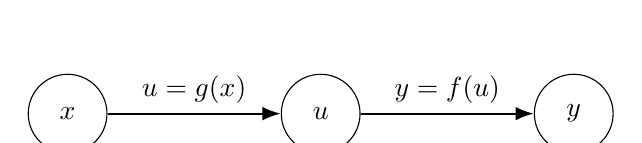
\begin{tikzpicture}[>=Latex,node distance=2.2cm]
\node[draw,circle,minimum size=10mm] (x) {$x$};
\node[draw,circle,minimum size=10mm,right=of x] (u) {$u$};
\node[draw,circle,minimum size=10mm,right=of u] (y) {$y$};
\draw[->,thick] (x) -- node[above] {$u=g(x)$} (u);
\draw[->,thick] (u) -- node[above] {$y=f(u)$} (y);
\end{tikzpicture}
\end{center}

여기에서 $u$는 단순한 기호가 아니라, $x$의 변화가 $y$로 전달되는 과정에 존재하는
\textbf{중간 변수(intermediate variable)}이다. 이 관점이 뒤에서 computational graph를 이해할 때 중요하다.

\subsection{Chain Rule}

$g$가 $x$에서 미분가능하고 $f$가 $g(x)$에서 미분가능하면
\[
h(x)=f(g(x))
\]
의 도함수는
\[
\boxed{
 h'(x)=f'(g(x))g'(x)
}
\]
이다.

중간 변수 $u=g(x)$를 사용하면
\[
\boxed{
\frac{dy}{dx}
=
\frac{dy}{du}\frac{du}{dx}
}
\]
로 쓸 수 있다.

\begin{thinkbox}[왜 ``곱''이 나타나는가?]
Chain rule을 단순한 공식으로 기억하기보다, \textbf{변화율의 전달}로 생각하는 것이 좋다.

$x$가 작은 양 $\Delta x$만큼 변할 때
\[
\Delta u \approx \frac{du}{dx}\Delta x
\]
이고, 이 변화가 다시 $y$에 전달되어
\[
\Delta y \approx \frac{dy}{du}\Delta u
\]
이다. 따라서
\[
\Delta y
\approx
\frac{dy}{du}\frac{du}{dx}\Delta x.
\]
한편 직접 $x$와 $y$의 관계만 보면
\[
\Delta y\approx \frac{dy}{dx}\Delta x
\]
이므로
\[
\frac{dy}{dx}=\frac{dy}{du}\frac{du}{dx}
\]
가 된다.
\end{thinkbox}

\begin{remarkbox}[직관: 톱니바퀴가 연결되어 있다고 생각하면]
$x$의 변화가 $u$를 두 배로 변화시키고,
\[
\frac{du}{dx}=2,
\]
$u$의 변화가 다시 $y$를 세 배로 변화시킨다면
\[
\frac{dy}{du}=3,
\]
$x$의 작은 변화는 최종적으로 $y$에 $2\times3=6$배의 변화를 만든다.
즉,
\[
\frac{dy}{dx}=\frac{dy}{du}\frac{du}{dx}=3\times2=6.
\]
이 비유의 핵심은 중간 변수 $u$를 거치면서 \textbf{변화율이 연쇄적으로 전달된다}는 데 있다.
\end{remarkbox}

이 관점에서 derivative는 단순한 기호 조작이 아니라
\[
\boxed{\text{입력의 작은 변화가 출력의 변화로 얼마나 증폭 또는 축소되는가}}
\]
를 나타내는 \textbf{sensitivity}이다.

\subsection{Local linearization으로 보는 미분}

미분가능한 함수 $f$는 $x$ 근처에서
\[
f(x+\Delta x)
=
f(x)+f'(x)\Delta x+o(|\Delta x|)
\]
로 근사된다. 즉,
\[
\boxed{\Delta f\approx f'(x)\Delta x}
\]
이다.

두 함수 $u=g(x)$, $y=f(u)$를 각각 선형근사하면
\[
\Delta u\approx g'(x)\Delta x,
\qquad
\Delta y\approx f'(u)\Delta u,
\]
따라서
\[
\Delta y\approx f'(g(x))g'(x)\Delta x.
\]
이것이 chain rule의 가장 중요한 구조이다.

\subsection{예제}

\paragraph{예제 1.}
\[
y=(x^3+1)^2.
\]
$u=x^3+1$이라 두면 $y=u^2$이므로
\[
\frac{dy}{dx}
=
\frac{dy}{du}\frac{du}{dx}
=
2u\cdot 3x^2
=
6x^2(x^3+1).
\]

\paragraph{예제 2.}
\[
y=\sin(2x+1).
\]
$u=2x+1$이라 두면
\[
\frac{dy}{dx}
=
\cos u\cdot 2
=
2\cos(2x+1).
\]

\paragraph{예제 3. 세 단계 합성}
\[
y=\exp\!\left(\sin(x^2)\right).
\]
중간 변수를
\[
u_1=x^2,\qquad u_2=\sin u_1,\qquad y=e^{u_2}
\]
로 두면
\[
\frac{dy}{dx}
=
\frac{dy}{du_2}
\frac{du_2}{du_1}
\frac{du_1}{dx}
=
e^{u_2}\cos u_1\,(2x).
\]
따라서
\[
\boxed{
\frac{dy}{dx}
=2x\cos(x^2)e^{\sin(x^2)}
}.
\]

\begin{mlbox}[Deep Learning을 향한 첫 번째 관찰]
합성 단계가 3개가 아니라 30개, 300개가 되어도 원리는 변하지 않는다.
\[
\frac{\partial L}{\partial x}
=
\frac{\partial L}{\partial u_m}
\frac{\partial u_m}{\partial u_{m-1}}
\cdots
\frac{\partial u_1}{\partial x}.
\]
Deep neural network는 이와 같은 긴 합성함수이다.
\end{mlbox}

% =================================================
\section{다변수 함수: Partial Derivative와 Gradient}
% =================================================

딥러닝의 loss는 일반적으로 하나의 변수만의 함수가 아니다. 모델이 $p$개의 parameter를 갖는다면
\[
L=L(\theta_1,\theta_2,\ldots,\theta_p)
\]
와 같은 다변수 함수이다.

\subsection{Partial derivative}

$f:\R^n\to\R$,
\[
f=f(x_1,\ldots,x_n)
\]
에 대해 $x_i$만 변화시키고 나머지 변수를 고정했을 때의 변화율을
\[
\frac{\partial f}{\partial x_i}
\]
라고 한다.

\subsection{Gradient}

이 노트에서는 optimization에서 흔히 사용하는 \textbf{column-vector convention}을 사용한다.
\[
\boxed{
\grad f(\vect{x})
=
\begin{bmatrix}
\dfrac{\partial f}{\partial x_1}\\[0.4em]
\vdots\\[0.2em]
\dfrac{\partial f}{\partial x_n}
\end{bmatrix}
\in\R^n
}
\]

그러면 다변수 함수의 1차 근사는
\[
\boxed{
 f(\vect{x}+\Delta\vect{x})
\approx
 f(\vect{x})
 +
 \grad f(\vect{x})\T\Delta\vect{x}
}
\]
이다.

즉,
\[
\Delta f
\approx
\sum_{i=1}^n
\frac{\partial f}{\partial x_i}\Delta x_i.
\]

\begin{thinkbox}[해석]
일변수의
\[
\Delta f\approx f'(x)\Delta x
\]
가 다변수에서는
\[
\Delta f\approx \grad f(\vect{x})\T\Delta\vect{x}
\]
로 일반화된다. Gradient는 모든 좌표방향의 sensitivity를 하나의 vector로 모은 것이다.
\end{thinkbox}

\subsection{예제: 두 변수 함수}

\[
f(x,y)=x^2+3xy+y^2.
\]
그러면
\[
\frac{\partial f}{\partial x}=2x+3y,
\qquad
\frac{\partial f}{\partial y}=3x+2y,
\]
따라서
\[
\grad f(x,y)
=
\begin{bmatrix}
2x+3y\\
3x+2y
\end{bmatrix}.
\]

$(x,y)=(1,2)$에서 $\Delta x=0.01$, $\Delta y=-0.02$라면
\[
\Delta f
\approx
\begin{bmatrix}8&7\end{bmatrix}
\begin{bmatrix}0.01\\-0.02\end{bmatrix}
=-0.06.
\]
즉, gradient는 작은 parameter 변화가 함수값에 어떤 변화를 주는지를 정량화한다.

% =================================================
\section{다변수 Chain Rule}
% =================================================

\subsection{여러 중간변수가 하나의 변수에 의존하는 경우}

\[
z=f(x_1,x_2,\ldots,x_n),
\qquad
x_i=x_i(t)
\]
라고 하자. 그러면 $z$는 결국 $t$의 함수이며
\[
\boxed{
\frac{dz}{dt}
=
\sum_{i=1}^n
\frac{\partial z}{\partial x_i}
\frac{dx_i}{dt}
}
\]
이다.

Gradient를 사용하면 더 간단히
\[
\boxed{
\frac{dz}{dt}
=
\grad_{\vect{x}}z\T
\frac{d\vect{x}}{dt}
}
\]
로 쓸 수 있다.

\begin{center}
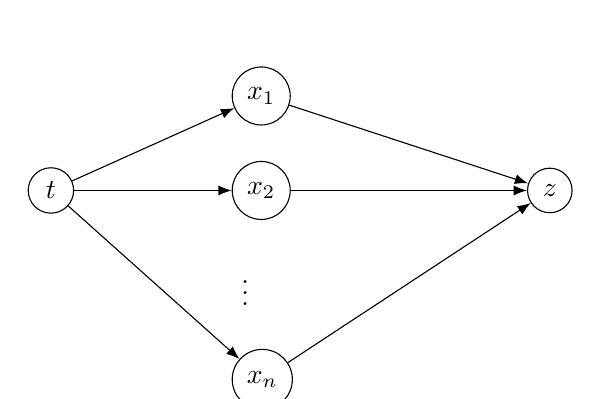
\begin{tikzpicture}[>=Latex,node distance=1.5cm and 2.0cm]
\node[draw,circle] (t) {$t$};
\node[draw,circle,right=of t,yshift=12mm] (x1) {$x_1$};
\node[draw,circle,right=of t] (x2) {$x_2$};
\node[right=of t,yshift=-12mm] (dots) {$\vdots$};
\node[draw,circle,right=of t,yshift=-24mm] (xn) {$x_n$};
\node[draw,circle,right=3.0cm of x2] (z) {$z$};
\draw[->] (t)--(x1);
\draw[->] (t)--(x2);
\draw[->] (t)--(xn);
\draw[->] (x1)--(z);
\draw[->] (x2)--(z);
\draw[->] (xn)--(z);
\end{tikzpicture}
\end{center}

$t$가 변하면 모든 $x_i$가 변하고, 각 $x_i$의 변화가 다시 $z$의 변화에 기여한다.
따라서 최종 변화율은 모든 경로(path)의 기여를 더한 값이 된다.

\subsection{예제}

\[
z=x^2+y^2,
\qquad
x=\cos t,
\qquad
y=\sin t.
\]
Chain rule에 의해
\[
\frac{dz}{dt}
=
2x\frac{dx}{dt}
+2y\frac{dy}{dt}
=
2\cos t(-\sin t)+2\sin t(\cos t)=0.
\]
실제로 $z=\cos^2t+\sin^2t=1$이므로 일치한다.

\subsection{여러 입력과 여러 출력: Jacobian}

이제
\[
\vect{u}=F(\vect{x}),
\qquad
F:\R^n\to\R^m
\]
인 vector-valued function을 생각하자. 즉,
\[
\vect{u}
=
\begin{bmatrix}
u_1\\ \vdots\\ u_m
\end{bmatrix},
\qquad
\vect{x}
=
\begin{bmatrix}
x_1\\ \vdots\\ x_n
\end{bmatrix}.
\]

$F$의 모든 편미분을 모은 행렬을 \textbf{Jacobian}이라 한다.
\[
\boxed{
J_F(\vect{x})
=
\begin{bmatrix}
\dfrac{\partial u_1}{\partial x_1} & \cdots & \dfrac{\partial u_1}{\partial x_n}\\[0.5em]
\vdots & \ddots & \vdots\\[0.3em]
\dfrac{\partial u_m}{\partial x_1} & \cdots & \dfrac{\partial u_m}{\partial x_n}
\end{bmatrix}
\in\R^{m\times n}
}
\]

그리고 local linearization은
\[
\boxed{
\Delta\vect{u}
\approx
J_F(\vect{x})\Delta\vect{x}
}
\]
이다.

\subsection{Jacobian 형태의 Chain Rule}

\[
\vect{x}\xrightarrow{F}\vect{u}\xrightarrow{G}\vect{y}
\]
라면
\[
\boxed{
J_{G\circ F}(\vect{x})
=
J_G(\vect{u})J_F(\vect{x})
}
\]
이다.

이 식은 local linearization만으로도 자연스럽게 이해할 수 있다. 먼저
\[
\Delta\vect{u}\approx J_F(\vect{x})\Delta\vect{x}
\]
이고, 다음 단계에서
\[
\Delta\vect{y}\approx J_G(\vect{u})\Delta\vect{u}
\]
이므로
\[
\Delta\vect{y}
\approx
J_G(\vect{u})J_F(\vect{x})\Delta\vect{x}.
\]
따라서 전체 합성함수의 1차 선형근사를 나타내는 Jacobian은 두 Jacobian의 곱이다.

이 식은 일변수 chain rule
\[
(g\circ f)'=g'(f)f'
\]
의 정확한 다변수 일반화이다.

\begin{remarkbox}[교재 표기와의 차이]
Deisenroth--Faisal--Ong의 \emph{Mathematics for Machine Learning}은 gradient를 row vector로 정의한다.
이 노트에서는 이후 optimization 및 neural-network 표기와의 연결을 위해 gradient를 column vector로 둔다.
두 표기 모두 가능하지만, 한 문서 안에서는 반드시 convention을 일관되게 유지해야 한다.
\end{remarkbox}

% =================================================
\section{Scalar Loss를 뒤로 미분하기: Backward의 핵심 식}
% =================================================

Deep learning에서 마지막 출력은 보통 하나의 scalar loss이다.
\[
\vect{x}
\xrightarrow{F}
\vect{u}
\xrightarrow{G}
L\in\R.
\]

$L=L(\vect{u})$이고 $\vect{u}=F(\vect{x})$라면 column-gradient convention에서
\[
\boxed{
\grad_{\vect{x}}L
=
J_F(\vect{x})\T
\grad_{\vect{u}}L
}
\]
이다.

이를 differential로 확인하면 더욱 분명하다. $\dd\vect{u}=J_F\dd\vect{x}$이고
\[
\dd L
=
\grad_{\vect{u}}L\T\dd\vect{u}
=
\grad_{\vect{u}}L\T J_F\dd\vect{x}
=
\left(J_F\T\grad_{\vect{u}}L\right)\T\dd\vect{x}.
\]
한편 정의에 의해 $\dd L=\grad_{\vect{x}}L\T\dd\vect{x}$이므로 위의 식을 얻는다.

이 식은 backpropagation을 이해하는 데 매우 중요하다. Forward에서는
\[
\Delta\vect{u}\approx J_F\Delta\vect{x}
\]
처럼 값의 변화가 왼쪽에서 오른쪽으로 전달되는 반면, backward에서는
\[
\grad_{\vect{x}}L=J_F\T\grad_{\vect{u}}L
\]
처럼 \textbf{loss의 sensitivity가 오른쪽에서 왼쪽으로 전달}된다.

\begin{mlbox}[Forward와 Backward]
\textbf{Forward propagation}: 현재 parameter를 이용하여 중간 변수와 출력, loss 값을 계산한다.

\textbf{Backward propagation}: loss가 각 중간 변수와 parameter에 얼마나 민감한지를 chain rule로 계산한다.

\[
\boxed{
\text{Forward: values flow forward}
\qquad
\text{Backward: gradients flow backward}
}
\]
\end{mlbox}

% =================================================
\section{Linear Regression을 Computational Graph로 다시 보기}
% =================================================

이제 이미 알고 있는 선형회귀를 chain rule의 관점에서 다시 해석한다.
데이터
\[
(x_i,y_i),\qquad i=1,\ldots,N
\]
가 주어졌다고 하자.

모델은
\[
\widehat y_i=wx_i+b
\]
이고, mean squared error는
\[
\boxed{
L(w,b)
=
\frac{1}{N}
\sum_{i=1}^N
(\widehat y_i-y_i)^2
}
\]
이다.

\subsection{한 개의 데이터에 대한 계산 그래프}

먼저 하나의 datum $(x,y)$만 생각하자.
\[
\widehat y=wx+b,
\qquad
e=\widehat y-y,
\qquad
\ell=e^2.
\]

\begin{center}
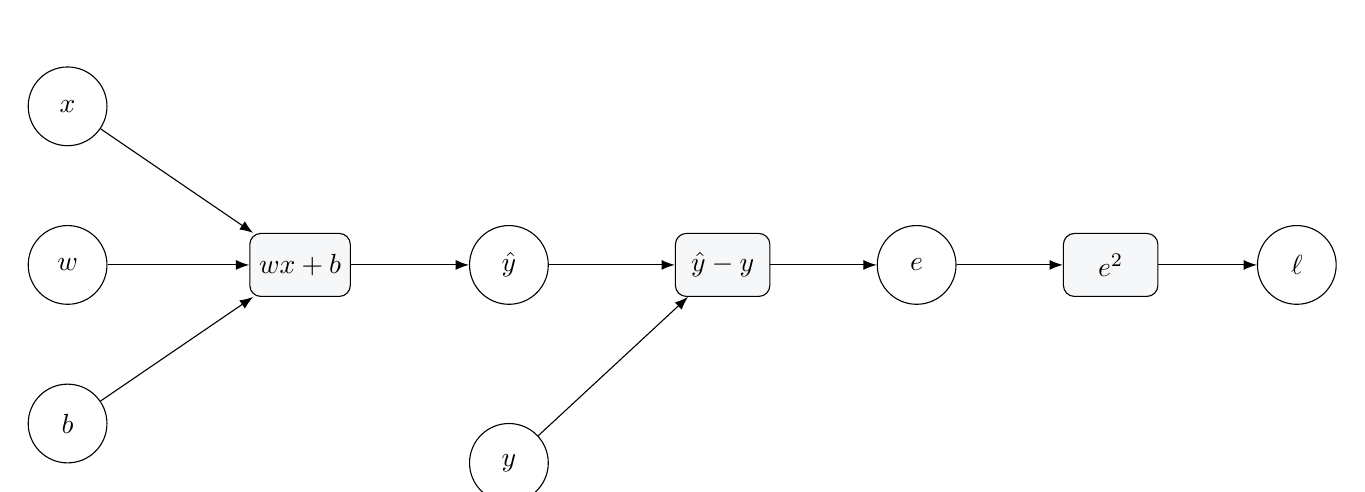
\begin{tikzpicture}[
>=Latex,
node distance=1.55cm and 1.6cm,
var/.style={draw,circle,minimum size=10mm,inner sep=1pt},
op/.style={draw,rounded corners,minimum height=8mm,minimum width=12mm,fill=softgray}
]
\node[var] (x) {$x$};
\node[var,below=10mm of x] (w) {$w$};
\node[var,below=10mm of w] (b) {$b$};
\node[op,right=1.8cm of w] (aff) {$wx+b$};
\node[var,right=1.5cm of aff] (yh) {$\hat y$};
\node[var,below=15mm of yh] (yt) {$y$};
\node[op,right=1.6cm of yh] (sub) {$\hat y-y$};
\node[var,right=1.35cm of sub] (e) {$e$};
\node[op,right=1.35cm of e] (sq) {$e^2$};
\node[var,right=1.25cm of sq] (ell) {$\ell$};
\draw[->] (x)--(aff);
\draw[->] (w)--(aff);
\draw[->] (b)--(aff);
\draw[->] (aff)--(yh);
\draw[->] (yh)--(sub);
\draw[->] (yt)--(sub);
\draw[->] (sub)--(e);
\draw[->] (e)--(sq);
\draw[->] (sq)--(ell);
\end{tikzpicture}
\end{center}

Forward 계산은 단순히
\[
(w,b,x)
\longrightarrow
\widehat y
\longrightarrow
e
\longrightarrow
\ell
\]
순서로 진행한다.

\subsection{Local derivatives}

각 edge에 해당하는 local derivative를 계산하면
\[
\frac{\partial \ell}{\partial e}=2e,
\qquad
\frac{\partial e}{\partial \widehat y}=1,
\]
그리고
\[
\frac{\partial \widehat y}{\partial w}=x,
\qquad
\frac{\partial \widehat y}{\partial b}=1.
\]

따라서 chain rule에 의해
\[
\boxed{
\frac{\partial \ell}{\partial w}
=
\frac{\partial \ell}{\partial e}
\frac{\partial e}{\partial \widehat y}
\frac{\partial \widehat y}{\partial w}
=
2ex
}
\]
이고
\[
\boxed{
\frac{\partial \ell}{\partial b}
=
\frac{\partial \ell}{\partial e}
\frac{\partial e}{\partial \widehat y}
\frac{\partial \widehat y}{\partial b}
=
2e
}
\]
이다.

즉, loss에서 시작하여 computational graph를 반대 방향으로 따라가면서
각 edge의 local derivative를 곱한다.

\subsection{전체 데이터에 대한 gradient}

\[
L(w,b)=\frac1N\sum_{i=1}^N\ell_i
\]
이므로
\[
\frac{\partial L}{\partial w}
=
\frac1N\sum_{i=1}^N
\frac{\partial \ell_i}{\partial w}
=
\boxed{
\frac{2}{N}\sum_{i=1}^N(\widehat y_i-y_i)x_i
}
\]
이고
\[
\frac{\partial L}{\partial b}
=
\boxed{
\frac{2}{N}\sum_{i=1}^N(\widehat y_i-y_i)
}
\]
이다.

Gradient vector는
\[
\grad L(w,b)
=
\begin{bmatrix}
\partial L/\partial w\\[0.2em]
\partial L/\partial b
\end{bmatrix}.
\]

Gradient descent는
\[
\boxed{
\begin{bmatrix}
w_{k+1}\\ b_{k+1}
\end{bmatrix}
=
\begin{bmatrix}
w_k\\ b_k
\end{bmatrix}
-
\eta
\begin{bmatrix}
\partial L/\partial w\\
\partial L/\partial b
\end{bmatrix}
}
\]
이다.

\begin{keybox}[여기에서 구분해야 할 두 가지]
\textbf{Backpropagation}은 gradient를 \emph{계산하는 방법}이다.

\textbf{Gradient descent}는 계산된 gradient를 사용하여 parameter를 \emph{업데이트하는 방법}이다.

즉,
\[
\boxed{
\text{Forward}
\rightarrow
\text{Loss}
\rightarrow
\text{Backward}
\rightarrow
\text{Gradient}
\rightarrow
\text{Parameter Update}
}
\]
이다.
\end{keybox}

% =================================================
\section{Matrix Form으로 한 번 더 보기}
% =================================================

선형회귀의 계산을 matrix form으로 쓰면 이후 neural network의 affine layer와 직접 연결된다.

\[
\vect{x}
=
\begin{bmatrix}
x_1\\ \vdots\\ x_N
\end{bmatrix},
\qquad
\vect{y}
=
\begin{bmatrix}
y_1\\ \vdots\\ y_N
\end{bmatrix}.
\]

Bias까지 포함한 design matrix와 parameter vector를
\[
X=
\begin{bmatrix}
x_1&1\\
\vdots&\vdots\\
x_N&1
\end{bmatrix},
\qquad
\vect{\theta}
=
\begin{bmatrix}w\\b\end{bmatrix}
\]
라 두면
\[
\widehat{\vect{y}}=X\vect{\theta}.
\]

Loss는
\[
L(\vect{\theta})
=
\frac1N\|X\vect{\theta}-\vect{y}\|_2^2
\]
이다. $\vect{e}=X\vect{\theta}-\vect{y}$라 두면
\[
L=\frac1N\vect{e}\T\vect{e},
\qquad
\dd\vect{e}=X\dd\vect{\theta}.
\]
따라서
\[
\dd L
=
\frac{2}{N}\vect{e}\T\dd\vect{e}
=
\frac{2}{N}\vect{e}\T X\dd\vect{\theta}
=
\left(\frac{2}{N}X\T\vect{e}\right)\T\dd\vect{\theta}.
\]
그러므로
\[
\boxed{
\grad_{\vect{\theta}}L
=
\frac{2}{N}X\T(X\vect{\theta}-\vect{y})
}
\]
이다.

이 한 줄을 성분별로 풀면 바로 앞 절의 $\partial L/\partial w$와 $\partial L/\partial b$가 나온다.

\begin{mlbox}[다음 단계와의 연결]
선형회귀의
\[
\widehat{\vect{y}}=X\vect{\theta}
\]
는 신경망 affine layer의
\[
A=XW+B
\]
와 본질적으로 같은 구조이다. 이후 MLP에서는 $W$와 $B$가 더 큰 matrix/vector가 되고,
그 사이에 activation function이 추가될 뿐이다.
\end{mlbox}

% =================================================
\section{숫자로 Gradient의 흐름을 끝까지 추적해 보기}
% =================================================

다음 세 개의 데이터를 생각하자.
\[
(1,1),\qquad(2,2),\qquad(3,2).
\]
초기값을
\[
w_0=1,\qquad b_0=1
\]
로 둔다. 그러면 $\widehat y=x+1$이다.

\begin{center}
\begin{tabular}{c|c|c|c|c|c|c}
\toprule
$x_i$ & $y_i$ & $\widehat y_i$ & $e_i$ & $\ell_i=e_i^2$ & $\partial\ell_i/\partial w$ & $\partial\ell_i/\partial b$\\
\midrule
1 & 1 & 2 & 1 & 1 & $2(1)(1)=2$ & $2(1)=2$\\
2 & 2 & 3 & 1 & 1 & $2(1)(2)=4$ & $2(1)=2$\\
3 & 2 & 4 & 2 & 4 & $2(2)(3)=12$ & $2(2)=4$\\
\bottomrule
\end{tabular}
\end{center}

따라서
\[
\frac{\partial L}{\partial w}
=
\frac{2+4+12}{3}=6,
\qquad
\frac{\partial L}{\partial b}
=
\frac{2+2+4}{3}=\frac{8}{3}.
\]

학습률을 $\eta=0.03$이라 하면 한 번의 gradient descent step은
\[
w_1=1-0.03(6)=0.82,
\]
\[
b_1=1-0.03\left(\frac83\right)=0.92.
\]

\begin{thinkbox}[학생에게 물어볼 질문]
\begin{enumerate}[label=(\arabic*)]
\item 왜 세 번째 데이터 $(3,2)$가 $w$의 gradient에 가장 큰 영향을 주는가?
\item $b$의 gradient에는 왜 $x_i$가 나타나지 않는가?
\item $e_i=0$인 데이터는 그 iteration에서 parameter update에 어떤 영향을 주는가?
\item $x_i$의 절댓값이 매우 크다면 $w$의 gradient 크기는 어떻게 될까?
\end{enumerate}
\end{thinkbox}

% =================================================
\section{3차시 실습: NumPy Hard Coding}
% =================================================

이번 실습에서는 PyTorch의 autograd를 사용하지 않는다.
수학적으로 유도한 모든 값을 직접 계산한다.

\subsection{실습 목표}

코드 안에서 다음 다섯 단계를 눈으로 확인한다.
\[
\boxed{
\text{data}
\rightarrow
\text{forward}
\rightarrow
\text{loss}
\rightarrow
\text{backward}
\rightarrow
\text{parameter update}
}
\]

\subsection{Step 1. 데이터와 모델}

\begin{lstlisting}
import numpy as np
import matplotlib.pyplot as plt

x = np.array([1., 2., 3., 4., 5.])
y = np.array([2.2, 2.8, 3.6, 4.5, 5.1])

w = 0.0
b = 0.0
learning_rate = 0.01
epochs = 200
N = len(x)
\end{lstlisting}

모델은
\[
\widehat y=wx+b
\]
이다.

\subsection{Step 2. Forward propagation}

\begin{lstlisting}
y_hat = w * x + b
error = y_hat - y
loss = np.mean(error**2)
\end{lstlisting}

이 세 줄은 수학적으로
\[
\widehat y_i=wx_i+b,
\qquad
e_i=\widehat y_i-y_i,
\qquad
L=\frac1N\sum_i e_i^2
\]
를 계산한다.

\subsection{Step 3. Backward propagation}

이번에는 최종 공식을 바로 쓰지 말고 local derivative를 코드에 그대로 남긴다.

\begin{lstlisting}
dl_de = 2.0 * error

de_dyhat = 1.0

dyhat_dw = x
dyhat_db = 1.0

# Chain rule for each sample
sample_grad_w = dl_de * de_dyhat * dyhat_dw
sample_grad_b = dl_de * de_dyhat * dyhat_db

# Mean over all samples
dL_dw = np.mean(sample_grad_w)
dL_db = np.mean(sample_grad_b)
\end{lstlisting}

수학식과 정확히 대응시키면
\[
\frac{\partial \ell_i}{\partial w}
=
\underbrace{\frac{\partial \ell_i}{\partial e_i}}_{2e_i}
\underbrace{\frac{\partial e_i}{\partial \widehat y_i}}_{1}
\underbrace{\frac{\partial \widehat y_i}{\partial w}}_{x_i}
\]
이고,
\[
\frac{\partial \ell_i}{\partial b}
=
\underbrace{\frac{\partial \ell_i}{\partial e_i}}_{2e_i}
\underbrace{\frac{\partial e_i}{\partial \widehat y_i}}_{1}
\underbrace{\frac{\partial \widehat y_i}{\partial b}}_{1}.
\]

\subsection{Step 4. Parameter update}

\begin{lstlisting}
w -= learning_rate * dL_dw
b -= learning_rate * dL_db
\end{lstlisting}

즉,
\[
w\leftarrow w-\eta\frac{\partial L}{\partial w},
\qquad
b\leftarrow b-\eta\frac{\partial L}{\partial b}.
\]

\subsection{Step 5. 전체 training loop}

\begin{lstlisting}
import numpy as np
import matplotlib.pyplot as plt

x = np.array([1., 2., 3., 4., 5.])
y = np.array([2.2, 2.8, 3.6, 4.5, 5.1])

w = 0.0
b = 0.0
learning_rate = 0.01
epochs = 200
N = len(x)

loss_history = []

for epoch in range(epochs):
    # ---------------------------------
    # 1. Forward
    # ---------------------------------
    y_hat = w * x + b
    error = y_hat - y
    loss = np.mean(error**2)

    # ---------------------------------
    # 2. Backward: local derivatives
    # ---------------------------------
    dl_de = 2.0 * error
    de_dyhat = 1.0
    dyhat_dw = x
    dyhat_db = 1.0

    sample_grad_w = dl_de * de_dyhat * dyhat_dw
    sample_grad_b = dl_de * de_dyhat * dyhat_db

    dL_dw = np.mean(sample_grad_w)
    dL_db = np.mean(sample_grad_b)

    # ---------------------------------
    # 3. Gradient-descent step
    # ---------------------------------
    w -= learning_rate * dL_dw
    b -= learning_rate * dL_db

    loss_history.append(loss)

    if epoch % 20 == 0:
        print(
            f"epoch={epoch:3d}, loss={loss:.6f}, "
            f"w={w:.4f}, b={b:.4f}, "
            f"dL_dw={dL_dw:.4f}, dL_db={dL_db:.4f}"
        )

print("final w =", w)
print("final b =", b)

# Plot fitted line
x_plot = np.linspace(0.5, 5.5, 100)
y_plot = w * x_plot + b

plt.figure(figsize=(10, 4))

plt.subplot(1, 2, 1)
plt.scatter(x, y, label="data")
plt.plot(x_plot, y_plot, label="fitted line")
plt.xlabel("x")
plt.ylabel("y")
plt.legend()
plt.grid(True)

plt.subplot(1, 2, 2)
plt.plot(loss_history)
plt.xlabel("epoch")
plt.ylabel("MSE loss")
plt.grid(True)

plt.tight_layout()
plt.show()
\end{lstlisting}

\subsection{Step 6. Gradient check: 우리가 유도한 미분이 맞는가?}

Backpropagation으로 계산한 gradient를 numerical differentiation과 비교해 볼 수 있다.

\begin{lstlisting}
def compute_loss(x, y, w, b):
    y_hat = w * x + b
    return np.mean((y_hat - y)**2)


def numerical_gradient(x, y, w, b, h=1e-5):
    dL_dw = (
        compute_loss(x, y, w + h, b)
        - compute_loss(x, y, w - h, b)
    ) / (2*h)

    dL_db = (
        compute_loss(x, y, w, b + h)
        - compute_loss(x, y, w, b - h)
    ) / (2*h)

    return dL_dw, dL_db
\end{lstlisting}

예를 들어 같은 $(w,b)$에서
\[
\left(\frac{\partial L}{\partial w},\frac{\partial L}{\partial b}\right)_{\text{backprop}}
\approx
\left(\frac{\partial L}{\partial w},\frac{\partial L}{\partial b}\right)_{\text{finite difference}}
\]
인지 확인한다.

\begin{remarkbox}[왜 gradient check가 중요한가?]
Neural network가 커지면 backward code는 훨씬 복잡해진다. 직접 유도한 gradient가 맞는지 확인하기 위해
작은 문제에서는 numerical differentiation을 기준값으로 사용할 수 있다.

하지만 numerical differentiation은 parameter마다 forward evaluation을 반복해야 하므로 실제 training 방법으로는 너무 비싸다.
Backpropagation은 모든 parameter의 gradient를 훨씬 효율적으로 계산한다.
\end{remarkbox}

% =================================================
\section{이번 주의 개념을 한 그림으로 정리}
% =================================================

\begin{center}
\begin{tikzpicture}[
>=Latex,
node distance=8mm,
box/.style={draw,rounded corners,minimum width=43mm,minimum height=9mm,align=center,fill=softgray}
]
\node[box] (c1) {일변수 Chain Rule\\$\dfrac{dy}{dx}=\dfrac{dy}{du}\dfrac{du}{dx}$};
\node[box,below=of c1] (c2) {다변수 Local Linearization\\$\Delta f\approx \nabla f\T\Delta\vect{x}$};
\node[box,below=of c2] (c3) {Jacobian Chain Rule\\$J_{G\circ F}=J_GJ_F$};
\node[box,below=of c3] (c4) {Scalar Loss의 Backward\\$\nabla_{\vect{x}}L=J_F\T\nabla_{\vect{u}}L$};
\node[box,below=of c4,fill=softgreen] (c5) {Linear Regression Backprop\\$\partial L/\partial w,\;\partial L/\partial b$};
\node[box,below=of c5,fill=softblue] (c6) {Gradient Descent\\$\theta\leftarrow\theta-\eta\nabla L$};
\draw[->,thick] (c1)--(c2);
\draw[->,thick] (c2)--(c3);
\draw[->,thick] (c3)--(c4);
\draw[->,thick] (c4)--(c5);
\draw[->,thick] (c5)--(c6);
\end{tikzpicture}
\end{center}

\begin{keybox}[이번 주의 한 문장]
\[
\boxed{
\text{학습은 loss를 parameter에 대해 미분하고, 그 gradient로 parameter를 바꾸는 과정이다.}
}
\]
그리고 여러 함수가 합성된 모델에서 그 gradient를 계산하게 해 주는 수학적 원리가 chain rule이다.
\end{keybox}

% =================================================
\section{연습문제}
% =================================================

\begin{enumerate}[label=\textbf{\arabic*.},leftmargin=2.2em]
\item 다음 함수의 도함수를 중간 변수를 명시하여 chain rule로 계산하라.
\[
y=\log\left(1+e^{2x}\right).
\]

\item
\[
z=x^2y+\sin y,
\qquad
x=t^2,
\qquad
y=e^t
\]
일 때 $dz/dt$를 구하라.

\item 다음 vector-valued function의 Jacobian을 구하라.
\[
F(x_1,x_2)
=
\begin{bmatrix}
x_1^2+x_2\\
\sin(x_1x_2)
\end{bmatrix}.
\]

\item 선형회귀에서 loss를
\[
L(w,b)=\frac{1}{2N}\sum_{i=1}^N(wx_i+b-y_i)^2
\]
로 정의하면 $\partial L/\partial w$, $\partial L/\partial b$는 어떻게 바뀌는가?
$1/2$를 붙이는 이유를 설명하라.

\item 데이터
\[
(1,2),\qquad(2,2),\qquad(4,5)
\]
와 초기값 $w=0$, $b=0$이 주어졌다고 하자. 한 번의 forward/backward를 직접 계산하여
$\partial L/\partial w$, $\partial L/\partial b$를 구하고, $\eta=0.05$로 한 번 update한 $(w,b)$를 계산하라.

\item 코드에서 $\texttt{learning\_rate}$를 $0.001$, $0.01$, $0.1$, $0.5$로 바꾸어 loss history를 비교하라.
학습률이 너무 작거나 너무 클 때 어떤 현상이 나타나는지 설명하라.
\end{enumerate}

% =================================================
\section*{다음 주 예고}
% =================================================

이번 주에는
\[
\widehat y=wx+b
\]
라는 선형모델을 다루었다. 다음 단계에서는 여기에 비선형 activation function을 붙인다.
\[
\boxed{
 x
\longrightarrow
 a=wx+b
\longrightarrow
 z=\phi(a)
}
\]
그러면
\[
\frac{\partial L}{\partial w}
=
\frac{\partial L}{\partial z}
\frac{\partial z}{\partial a}
\frac{\partial a}{\partial w}
\]
와 같이 chain rule이 한 단계 더 길어진다.
이 구조가 neuron이며, 여러 neuron과 여러 layer를 연결하면 MLP의 backpropagation으로 자연스럽게 확장된다.

\section*{참고문헌}
\begin{itemize}
\item M. P. Deisenroth, A. A. Faisal, C. S. Ong, \emph{Mathematics for Machine Learning}, Cambridge University Press, Chapter 5 (Vector Calculus), especially Sections 5.2, 5.3, and 5.6.
\end{itemize}

\end{document}
